%% 和文論文用のテンプレート
%%%%%%%%%%%%%%%%%%%%%%%%%%%%%%%%%%%%%%%%%%%%%%%%%%%%%%%%%%%%%%%%%%%%%%%%%%%%
%% 1. 和文原稿
% \documentclass[originalpaper]{jsaiart}     % 原著論文 Original Paper
%\documentclass[blindreview]{jsaiart}      % 査読用
%
% \documentclass[shortpaper]{jsaiart}       % 速報論文 Short Paper
\documentclass[exploratorypaper]{jsaiart} % 萌芽論文 Exploratory Research Paper
% \documentclass[Specialissue]{jsaiart}     % 特集 Special Issue
% \documentclass[specialissue]{jsaiart}     % 小特集 Special Issue
% \documentclass[interimreport]{jsaiart}    % 報告 An Interim Report
% \documentclass[surveypaper]{jsaiart}      % 解説 Survey Paper
% \documentclass[aimap]{jsaiart}            % AIマップ AI map
% \documentclass[specialpaper]{jsaiart}     % 特集論文 Special Paper
% \documentclass[invitedpaper]{jsaiart}     % 招待論文 Invited Paper
%

%\usepackage{graphics}
\usepackage[dvipdfmx]{graphicx}
\usepackage{url}
%\usepackage[dvipdfmx]{profile-2e}

%% ページ番号の指定,掲載時に学会の方で決定します.
% \setcounter{page}{1}
% \setcounter{volpage}{1}


%%% amsmathパッケージの注意点 %%%%%%%%%%%%%%%%%%%%%%%%%%%%%%%%%%%%%%%
% \usepackpage{amsmath}
% 数式番号の参照は \ref ではなく,\eqref を用いること
% documentclass のオプションに fleqnを指定すること
% 例: \documentclass[technicalpaper,fleqn]{jsaiart}

\Vol{12}
\No{1}
\jtitle{一般化のためのネットワークプログラミング}
% \jtitle[柱用和文タイトル]{和文タイトル}

%\jsubtitle{論理的推論によるビットNOT演算プログラムの獲得}
%\jsubtitle{帰納推論による汎用プログラムの獲得}
\jsubtitle{帰納推論による任意プログラム獲得に向けての提案}
\etitle{NP4G : Network Programming for Generalization}
%\esubtitle{Acquisition of a bitwise NOT operator's program by logical inference}
%\esubtitle{Acquisition of a general-purpose program by inductive inference}
\esubtitle{The proposal toward acquisition of any programs by inductive inference}

% \manyauthor % 著者が3名以下の場合はこの行を消すこと

%%% 著者名の注意点 %%%%%%%%%%%%%%%%%%%%%%%%%%%%%%%%%%%%%%%%%%%%%%%%%%%
% 所属先が同じ著者が連続する場合,その中の先頭の著者のみ \affiliation
% を用い,残りの所属先には \sameaffiliation を使う
% ただし,所属先が同じでも連続していない場合は \affliation を使う
% 名前が長い場合は \name の代りに \longname を使う

\author{%
 \name{原}{匠一郎}{Shoichiro Hara}
 \affiliation{名古屋市立大学}%
     {Nagoya City University}%
     {s.hara@nsc.nagoya-cu.ac.jp}
\and
 \name{渡邊}{裕司}{Yuji Watanabe}
 \sameaffiliation{yuji@nsc.nagoya-cu.ac.jp}
}

\begin{keyword}
inductive inference, automatic programming, knowledge acquisition, GP, GNP
\end{keyword}

\begin{summary}
 In this study, we propose NP4G : Network Programming for Generalization. NP4G is available on GitHub\footnotemark[1].
\end{summary}

\begin{document}
\maketitle
\footnotetext[1]{公開予定}
\section{はじめに}
コンピュータプログラムを自動生成する自動プログラミングの研究は,長く活発に研究がされている分野であり,遺伝的プログラミングをはじめとして,さまざまなアプローチによる研究が行われてきた.近年では,GPT-3などニューラルネットワークを用いた自動プログラミングの研究が活発に行われており,注目を集めている.しかしニューラルネットワークを用いた手法は,論理的推論という点において,課題が残る.また,他の論理的な推論を行う手法であっても,依然として,任意プログラムに対して,論理的な推論によって自動生成するようなシステムの実現には至っていない.
%また,人工知能における論理的推論に関する研究は歴史が長く,エキスパートシステムをはじめとして,さまざまなアプローチによる研究が行われてきた.しかし依然として,あらゆる知識に対し自ら学習をし,その内容を活かして別の問題に対して論理的に推論し答えを導くような,汎用的で柔軟な人工知能の実現には至っていない.
%近年のニューラルネットワークを活用した人工知能の発達はめざましいが,論理的推論という点において,課題が残る.
一方で,知識獲得に関する研究は,知識獲得問題が顕著に表れるようになった頃から,あまり研究がされなくなっていった.
しかし人工知能研究の発展にはこのどちらも重要であり,

特に1つ1つの事例から論理的推論によって一般化を行う帰納推論は,知識獲得において,重要な課題である.

%人工知能という言葉が初めてできたダートマス会議での提案書の序文には,「機械が言語を使うことができるようにする方法の探究,機械上での抽象化と概念の形成,今は人間にしか解けない問題を機械で解くこと,機械が自分自身を改善する方法などの探究の試みがなされるだろう」と書かれているが\cite{dartmouth},.

本研究では,論理的推論の1つである帰納推論によってプログラムを自動生成することができる,一般化のためのネットワークプログラミング(NP4G: Network Programming for Generalization)を提案する.これは,プログラミングにおける順次,選択,繰り返しの構築が実現できる手法であることから,構造化定理を満たし,任意プログラムを帰納推論によって自動的に獲得することが期待できる手法といえる.なお,本研究で用いたプログラムのソースコードはGitHub上で一般公開している\footnotemark[1].

%これは,帰納推論に限らず,ネットワークプログラミングという新しい分野の方向性を示したものであるともいえる.

\section{関連研究}
本研究では,一般化のためのネットワークプログラミングを提案する.この目的と関連した研究として,(1)遺伝的プログラミング,(2)帰納推論,(3)自動プログラミングに関する研究を紹介する.
\subsection{遺伝的プログラミング}
類似研究として,GNPが挙げられる.
GPは木構造のみを扱うが,これをネットワークに拡張したものが遺伝的ネットワークプログラミング(GNP:Genetic Network Programming)である\cite{gnp}.

GP/GNPでは各ノードを単純な処理をする最小単位と考え,それらを木構造状またはネットワーク状に接続することによりプログラムを構築する.
GNPは遺伝的操作によりプログラムを自動生成できる機能を持つ.

ネットワークにすることで,それぞれのノードの組み合わせで,プログラムを自動的に構築することができる.

判定ノード,処理ノード,スタートノードに分類することができる.

%\subsection{論理的推論}
\subsection{帰納推論}
広義に論理的推論は,演繹的推論と帰納的推論,類比的推論の3つで構成されている(『算数・数学科重要用語300の基礎知識』p.106).
論理的思考の代表的なものとして「帰納的な考え方」,「類推的な考え方」,「一般化の考え方」,「記号化の考え方」などがある\cite{saito:11}.

ニューラルネットワークの手法では,確かに個々のデータの特徴の共通点を拾い出すことができるため,その点においては一般化ができると言えるが,膨大なデータに基づいて相関関係を求めたものであり,論理的でない.
また,その判断プロセスは説明可能性に乏しく,この問題はブラックボックス問題と呼ばれている[出典].ある程度の分析はできるものの[出典],明確な重みづけの基準を理解することは非常に困難である.

ニューラルネットワークでは原因と効果や,なぜ関連性や相関があるのかを解釈できない.特に,創造や計画,推論を伴うタスクは得意としない.これと同様に,AIが学習を一般化することに限界がある.一般化の欠如は大きい問題である.
また,学習には大量のデータが必要であり,このことからも帰納推論でないことがわかる.

ベイズモデルを用いた手法も報告されている\cite{TENENBAUM2006}.
パターンの規則を用いた論理的推論であるパターン推論の手法が報告されている\cite{tsukimoto:00}\cite{sudo:07}.
%このように,論理的推論の手法はいくつか提案されているが,論理的推論における一般化の手法は見つからない.
%->帰納推論という用語で,論理的推論における一般化の手法が考案されている.


帰納推論は知識獲得とも深い関連がある.
知識獲得問題がある\cite{KnowledgeAI}[知識の獲得と学習][他の出典].
\subsection{自動プログラミング}
Logic Theorist\cite{LogicTheorist}は探索木とヒューリスティクスを利用し,人間の論理的推論を模倣することを意図して作られた.

最近では,GPT3\cite{gpt3}などの手法を用いた自動プログラミングのように,一般に公開されている膨大なコードから学習をし,開発者の書こうとしているコードを予測して,その続きを提案するような機能も出てきている\cite{copilot}.
%プログラミングの補完機能

これらは言語生成アルゴリズムであり,帰納推論によりコードを生成しているわけではない.

\section{提案手法}
\subsection{NP4Gの基本概念}
NP4Gは,教師データに基づき,ネットワークで表現されるプログラムを自動生成することで,帰納推論を行う手法である.教師データは,1入力1出力のデータであり,その教師データに合致する入出力が得られるプログラムが生成されるまで探索を行う.生成されるプログラムは,遺伝的ネットワークプログラミング(GNP)の考え方に基づき,簡単な機能を持った複数の素子をネットワーク状に接続することで得られる.GNPは遺伝的手法を用いたネットワークプログラミングであるが,NP4Gは遺伝的手法を用いるに限らない手法であり,さまざまな手法への応用を想定している.
%また帰納推論に用いる手法は例がない.->例がないなどは言わなくて良い

また,NP4Gは,1つ1つの事例(教師データ)に対して一般化を行うことで,1つの知識(プログラム)を獲得するという点において,帰納学習による知識獲得といえる.

(この文脈において,NP4Gは知識獲得問題を解決する手法になり得るといえる.)

また,NP4Gは帰納推論手法であるため,ニューラルネットワークなどを使った手法と違い,一般化をするために必要な教師データの数は一般化する対象の特徴が掴める程度(数個程度)と,非常に少なく済む.加えて,構築されたプログラム自体がネットワークの形になっているため,内部でどのような処理をしているのか明らかである.

ネットワークの組み合わせにより,自動でプログラムを生成する試みは,従来,遺伝的手法でのみ使用されてきたが,本研究ではネットワークプログラミングを,一般化をするための手段として用いる.この遺伝的手法に限らないネットワークプログラミングは,新しい自動プログラミング手法として,今後新しい分野として幅広く応用されると期待できる(ネットワークプログラミングの何がすごくて,どこがいいのか,理由を書く).

今後,GP/GNPと同じく,ニューラルネットワークや強化学習等の他の手法との組み合わせによる効果的なアルゴリズムの拡張が期待できる.

任意のプログラムを得るためには,構造化定理を満たすような手法であれば良いといえる.構造化定理とは,いかなるプログラムも、3種類の基本構造、「順次」、「選択」、「繰り返し」の組み合わせによって構成できると主張する定理である\cite{StructuredProgramming}.NP4Gは,スタートノードから決められた順序によってノードを実行することで「順次」を,予め与えられる関数を工夫することで「選択」を,イテラブルなデータによって「繰り返し」を実現できることから,構造化定理を満たすといえる.
自動定義関数(ADFs),段階的学習を用いる.

\begin{figure*}[t]
    \begin{center}
        %\includegraphics[width=90mm]{ab0ex-mtphu.eps}
        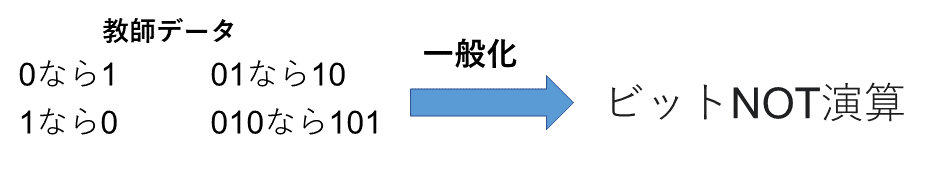
\includegraphics[width=90mm]{summary.jpg}
        %\epsfile{file=ab0ex-mtphu.eps,width=90mm}
    \end{center}
    \capwidth=90mm %
    \caption{NP4Gの概要}
    \label{fig:summary}
\end{figure*}

\subsection{NP4Gの基本構造}
%\subsection{NP4Gの構造}
NP4Gは\ref{fig:sequence}のように,複数の関数やオブジェクトといったノードがネットワーク状に接続された有効グラフ構造を持つ.入力として接続されるリンクの数は関数によって違うが,出力のリンクの数は関数によらず何本でも接続できる.
%GP,GNPでは,エージェントの行動をシミュレートする目的で使用する場合,処理ノードで
%(NP4Gでは,入力と出力データのペアである教師データをもとに推論を行うモデルであり,GNPで見られるような遅れ時間を設定する必要はない.)
%\subsubsection{ノードの実行順序}
%\subsubsection{ネットワークの自動生成}

NP4Gで生成されるネットワークの実行順序を説明する.
\ref{fig:sequence}に示すように,入力データを持つスタートノードから出るリンクに接続されているノードが,上から順に実行されていく.
処理が始まり,出力リンクをたどり,順番に関数が実行され,最後に実行された関数の出力が,そのネットワーク全体の出力となる.
入力ノードがまだ計算されておらず,結果が出力されていない場合,「not yet」なりスキップされる.また,すでに計算され結果が出力されているノードが再び選択された場合もスキップされる.

ノードは関数,スタートノード,オブジェクトに大別される.

\begin{figure*}[t]
    \begin{center}
        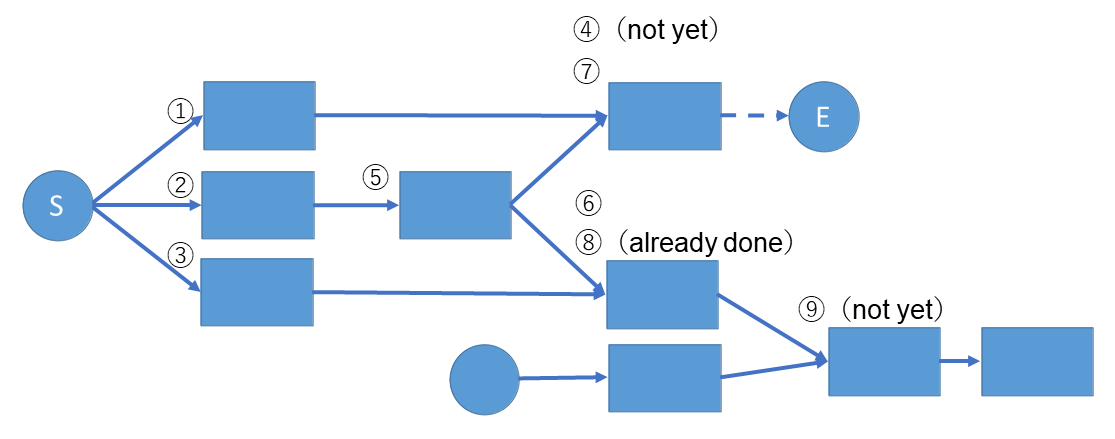
\includegraphics[width=130mm]{sequence.png}
    \end{center}
    \capwidth=90mm %
    \caption{NP4Gの実行順序}
    \label{fig:sequence}
\end{figure*}

\subsubsection{繰り返し処理}
より表現力の高い計算モデルを構築するためには,繰り返し処理を導入する必要がある.NP4Gでは,繰り返し処理を,ネットワーク上にフィードバックループを設けることで実現するのではなく,[]のようにイテラブルなデータを関数に入力させることで実現する.入力としてイテラブルなデータが与えられた関数は,そのデータの要素ごとに同じ処理を実行する.こうすることで,無限ループに陥り終了することのないプログラムが作成されることなく繰り返し処理を実現することができる.イテラブルなデータの生成あるいはイテラブルでないデータに戻す処理も関数が行い,イテラブルなデータが関数の入力として用いられる限り繰り返し処理がなされる.

\subsubsection{自動定義関数(ADFs)}
GPでは,プログラムの進化の際に高速化が望めるなどの理由から自動関数定義(ADFs:Automatically Defined Functions)\cite{adfs}が用いられる.ADFsはGPの性能を向上させる目的で,問題に存在するモジュール性を利用する方法である.
すでに出来上がったネットワークを再利用することで,より高度なプログラムを短時間のうちに作成することが可能になる.
予め定められたネットワーク構造のNP4G(一般化のためのネットワーク型プログラミング)を実行する。個々のADFsはlambda関数を使って定義し、ADFsリストに追加する。


\subsubsection{段階的学習}
段階的学習(Phased learning)は主に強化学習で用いられる手法である\cite{hodohara2012reinforcement}.
簡単なプログラムから段階的にネットワークを得て,ADFsとして次にネットワークを構築するときの材料として再利用することで,はじめから複雑なネットワークを得るときよりも短時間で学習をすることができる.
人間の学習でも,最初は簡単なレベルの学習から始め,徐々に難易度を上げていくと,無理なく学習できる.

\section{ビットNOT演算プログラムの獲得}
NP4Gを使って,ビットNOT演算プログラムを自動で構築する場合を考える.

\subsection{設定}
NP4Gを用いて,ビットNOT演算プログラムを獲得する実験を行った.
Python(Python 3.7.12)を使ってプログラムを作成した.繰り返し処理を実現するためのイテラブルなデータとして,Pythonプログラム上でリスト型のオブジェクト(以下,リスト)を使用した.
データは文字列で表記する.

\begin{table}[htbp]
\centering
\caption{学習に用いる教師データのすべて}
\label{tbl:result}
\begin{tabular}{l}
    \hline
     ( 入力 , 出力 ) \\
    \hline \hline
    ( "0" , "1" ) \\
    ( "1" , "0" ) \\
    ( "0 0" , "1 1" ) \\
    ( “0 1 0” , ”1 0 1” ) \\
    \hline
\end{tabular}
\end{table}

\subsection{段階的学習の方法}
以下の入出力を得るネットワークをADFsリストに登録する.

%1. “0”の入力に対して”1”の出力

%2. ”1”の入力に対して“0”の出力

%3. “0”の入力に対して”1”の出力,”1”の入力に対して“0”の出力

%4. “0”の入力に対して”1”の出力,”1”の入力に対して“0”の出力,“0 0”の入力に対して”1 1”の出力

%5. “0”の入力に対して”1”の出力,”1”の入力に対して“0”の出力,“0 0”の入力に対して”1 1”の出力,“0 1 0”の入力に対して”1 0 1”の出力

段階1. (“0”,”1”)

段階2. (”1”,“0”)

段階3. (“0”,”1”), (”1”,“0”)

段階4. (“0”,”1”), (”1”,“0”), (”0 0”,“1 1”)

段階5. (“0”,”1”), (”1”,“0”), (”0 0”,“1 1”), (”0 1 0”,“1 0 1”)


段階的学習の影響:3段階,4段階,5段階の3つを比較
3段階:段階2,3,4
4段階:段階1,2,3,4
5段階:段階1,2,3,4,5

\subsection{与えられる関数}
\subsubsection{split関数}
スペースを区切りとして,文字列を分けリスト表記にする.図で示すときは「split」を四角で囲い表記している.

%\begin{figure}[t]
%    \begin{center}
%        %\includegraphics[width=90mm]{ab0ex-mtphu.eps}
%        \includegraphics[width=50mm]{div.png}
%        %\epsfile{file=ab0ex-mtphu.eps,width=90mm}
%    \end{center}
%    \capwidth=50mm %
%    \caption{図の説明文... }
%\end{figure}

\subsubsection{sum関数}
リスト型の入力やそれ以外の文字列など,複数の入力に対し平滑化を行い,文字列との間をスペースで挟んで結合することで1つの文字列にする.入力の文字列が"[NuLL]"である場合,"[NuLL]"は結合しない.出力の文字列が""である場合,"[NuLL]"を出力する.図で示すときは「+」を四角で囲い表記している.

\subsubsection{equal関数}
2本の入力の値が一致するとき"[TRUE]"を出力する.それ以外は"[FALSE]"を出力する.GP/GNPでいう判定ノードの役割を果たす.図で示すときは「==」を四角で囲い表記している.

\subsubsection{制御ゲート関数}
2本の入力のうち,どちらかが"[TRUE]"である場合は,もう片方の入力の値を通し,それ以外は"[NULL]"を出力する.GP/GNPでいう処理ノードの役割を果たす.図で示すときは白丸で表記している.

\begin{figure*}[t]
    \begin{center}
        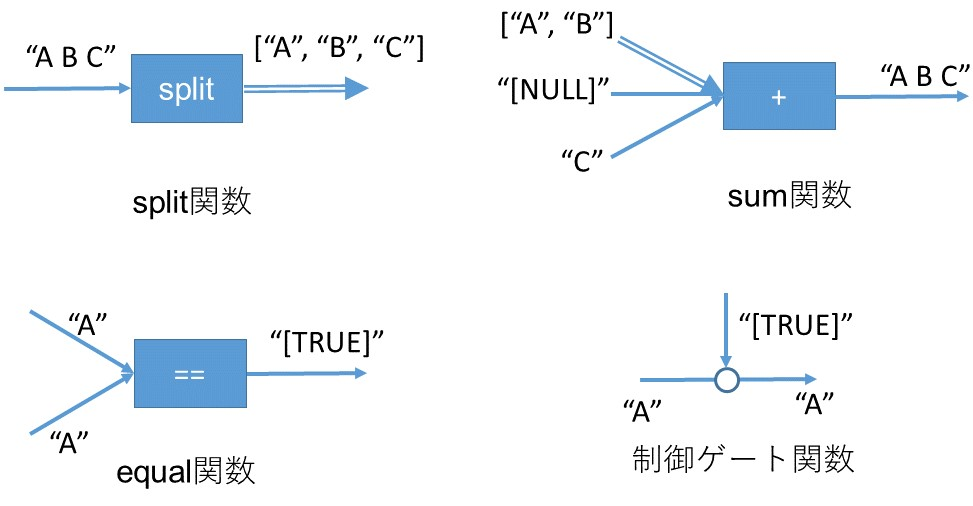
\includegraphics[width=110mm]{func.jpg}
    \end{center}
    \capwidth=90mm %
    \caption{予め与えられる関数}
    \label{fig:func}
\end{figure*}

\begin{figure*}[t]
    \begin{center}
        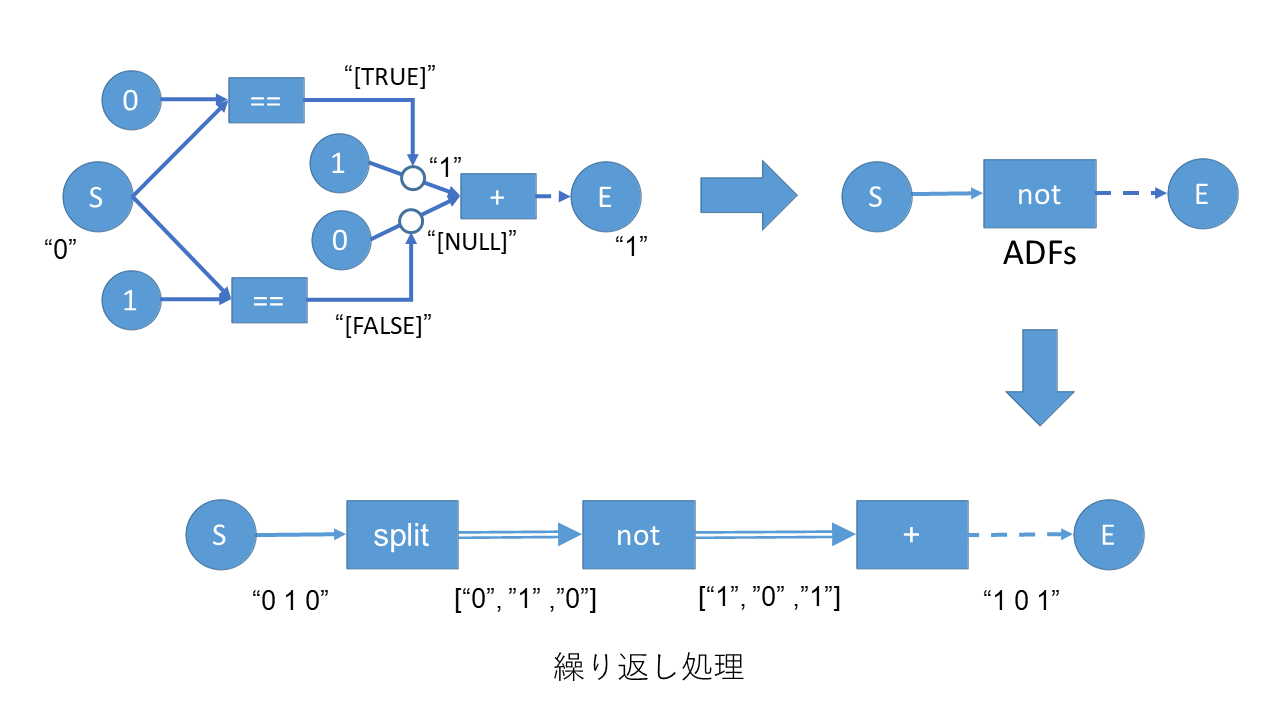
\includegraphics[width=150mm]{bitwise_not.png}
    \end{center}
    \capwidth=130mm %
    \caption{ビットNOT演算プログラムの実現例.このように段階を踏んでネットワークを構築することで,目的のプログラムを実現する(段階的学習).ADFsにより,最初に作った論理NOTプログラムのネットワークを次のネットワーク構築に再利用する.繰り返し処理はイテラブルなデータ(リスト)によって行われる.}
    \label{fig:bitwise_not}
\end{figure*}

ビットNOT演算プログラムを自動で構築するプログラムを10回実行する.
\section{結果と考察}
1桁から5桁までのすべての2進数の文字列(”0”から”1 1 1 1 1”)を使って,生成されたプログラムを検証した.
10回繰り返し,その実行時間の平均値を求めた.
制限時間は3時間(10800秒)

3段階から5段階まで段階的学習の段階の数を変化させたときの生成結果と実行時間の結果を\ref{tbl:result1},\ref{tbl:result2},\ref{tbl:result3}に示す.また,各段階における平均時間の結果を\ref{tbl:result4}に示す.3段階から5段階までのすべての生成結果を見ると,失敗したネットワーク(教師データの条件はすべて満たすが検証結果を満たさない)は段階的学習が4段階,ノード数が10個のときの1例のみだった.時間内に終わりやすいのは,段階的学習が3段階,ノード数が10個のときだった.
ノード数5のときの生成結果を見ると,5段階のときの成功の1例のみを除いて,すべて時間超過となった.
\ref{tbl:result4}からわかるように,段階3の学習時間が2585.24(s)と最も高くなっている.この原因は,段階3が「(“0”,”1”), (”1”,“0”)」の学習であり,1つのネットワークで初めて,2つの条件を満たすネットワークを探索する必要があることから,学習コストが高くなったためと考えられる.
\ref{fig:out_net_p5n5}に5段階ノード数5での自動生成によって期待するプログラムが得られたときのネットワークを示す.段階4の時点でビットNOT演算プログラムが得られていることを確認している.
\ref{fig:out_net_p4n10}に4段階ノード数10での自動生成によって,学習に用いた教師データと入出力は一致したが,期待と異なるプログラムが得られたときのネットワークを示す.このネットワークの場合,”0 1 0”の入力に対して“1 0 1”でない出力となった.このように,教師データと入出力が一致するネットワークが生成されたとしても,期待するネットワークが得られない場合もあることがわかる.この場合でも,段階を増やし,(”0 1 0”,“1 0 1”)も含めた教師データによって学習することで,改善を図ることができる.

%\begin{table}[htbp]
%\centering
%\begin{center}
%\end{tabular}
%\end{center}
%\end{table}

\begin{table}[t]
\caption{3段階の段階的学習の生成結果と実行時間(s)}
\label{tbl:result1}
\begin{tabular}{c|cccc}
    ノード数&	5&	10&	15&	20\\
    \hline
    成功&	0&	8&	6&	2\\
    失敗&	0&	0&	0&	0\\
    超過&	10&	2&	4&	8\\
    \hline \hline
    平均時間&	- &	3067.23&	5564.88&	3699.22\\
    最大時間&	0.00&	10480.28&	8966.41&	9542.54\\
    最小時間&	0.00&	258.23&	1.19&	3.24\\
    \hline
\end{tabular}
\end{table}

\begin{table}[t]
\caption{4段階の段階的学習の生成結果と実行時間(s)}
\label{tbl:result2}
\begin{tabular}{c|cccc}
    ノード数&	5&	10&	15&	20\\
    \hline
    成功&	0&	7&	6&	7\\
    失敗&	0&	1&	0&	0\\
    超過&	10&	2&	4&	3\\
    \hline \hline
    平均時間&	-&	3023.63&	334.40&	1104.84\\
    最大時間&	0.00&	8293.86&	1102.60&	2834.49\\
    最小時間&	0.00&	133.70&	6.46&	9.77\\
    \hline
\end{tabular}
\end{table}

\begin{table}[t]
\caption{5段階の段階的学習の生成結果と実行時間(s)}
\label{tbl:result3}
\begin{tabular}{c|cccc}
    ノード数&	5&	10&	15&	20\\
    \hline
    成功&	1&	6&	7&	5\\
    失敗&	0&	0&	0&	0\\
    超過&	9&	4&	3&	5\\
    \hline \hline
    平均時間&	32.18&	4089.67&	1505.77&	1265.54\\
    最大時間&	32.18&	9103.33&	7866.33&	2585.50\\
    最小時間&	32.18&	0.75&	2.29&	26.04\\
    \hline
\end{tabular}
\end{table}

\begin{table}[t]
\caption{各段階における平均時間(s)}
\label{tbl:result4}
\begin{tabular}{c|ccccc}
    段階&	1&	2&	3&	4&	5\\
    \hline
    平均時間&	1.17&	2.24&	2585.24&	188.31&	12.49\\
\end{tabular}
\end{table}


%\begin{figure*}[t]
%    \begin{center}
%        %\includegraphics[width=90mm]{ab0ex-mtphu.eps}
%        \includegraphics[width=120mm]{network.jpg}
%        %\epsfile{file=ab0ex-mtphu.eps,width=90mm}
%    \end{center}
%    \capwidth=90mm %
%    \caption{図の説明文... }
%    \label{fig:net}
%\end{figure*}

\begin{figure*}[t]
    \begin{center}
        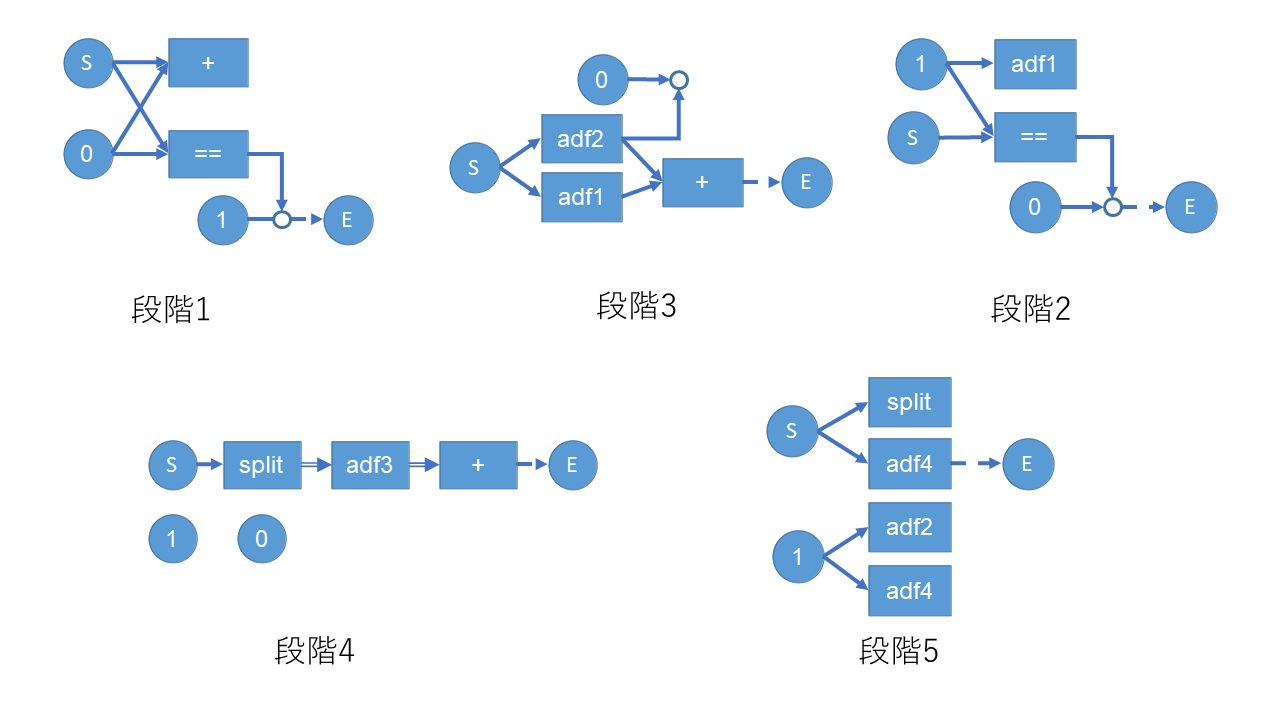
\includegraphics[width=150mm]{out_net_p5n5.png}
    \end{center}
    \capwidth=90mm %
    \caption{5段階ノード数5での自動生成によって期待するプログラムが得られたときのネットワーク}
    \label{fig:out_net_p5n5}
\end{figure*}

\begin{figure*}[t]
    \begin{center}
        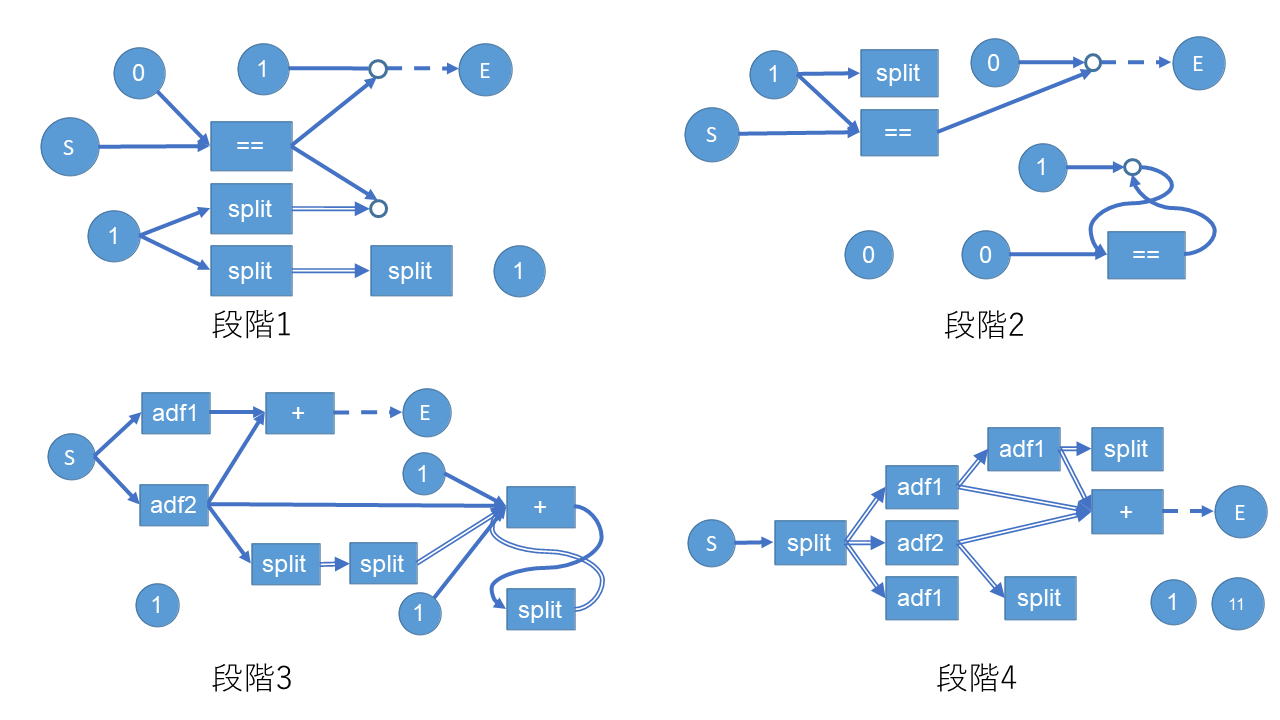
\includegraphics[width=150mm]{out_net_p4n10.png}
    \end{center}
    \capwidth=90mm %
    \caption{4段階ノード数10での自動生成によって,学習に用いた教師データと入出力は一致したが,期待と異なるプログラムが得られたときのネットワーク}
    \label{fig:out_net_p4n10}
\end{figure*}

\section{おわりに}
本研究では,一般化のためのネットワークプログラミング(NP4G)を提案した.NP4Gを使うことで,数個の教師データからビットNOT演算プログラムを獲得することに成功した.
NP4Gの過程(工程,計算アルゴリズム)は,数個の事例から一般的な性質を見出していくものであり,すなわち,帰納推論であるといえる.
これは知識獲得問題を解決する手法として期待できる.
ネットワークプログラミング(NP)という新しい分野の方向性を示した.
\subsection{まとめと本研究の意義}
本研究の意義は,ネットワークプログラミング(NP)によって,あらゆる知識に対し自ら学習をし,その内容を活かして別の問題に対して論理的に推論し答えを導くような,汎用的で柔軟な人工知能の実現が期待できることを示した点にある.
\subsection{今後の課題}
\subsubsection{チューリング完全性}

ビットNOT演算子だけでなく,他のプログラムもNP4Gを使って自動で構築できるか試してみる必要がある.

チューリング完全であることを証明することができれば,広く自動プログラミングとして応用可能であることが理論的に示すことができる.
しかし構造化定理によって,現時点でも,すべてのプログラムに対応可能であるとほぼいえる.
\subsubsection{探索手法の模索}
本研究では,ネットワークの探索方法として,ランダムな生成による偶発的な探索手法を用いた.この手法はプリミティブな手法であり,より効率の良い探索手法を模索する余地が残る.用いるノードの種類や数が増えるほど,探索に時間がかかる.今後,強化学習を用いるなどすることで,ネットワークを構築するのに最適なノードの種類や数,組み合わせ方を自動で調整できることが期待される.
\subsubsection{ネットワークの評価}
遺伝的手法に限らず,何らかの探索手法を用いる場合,生成された個体の評価を行う必要がある.本研究では,目的のネットワークが生成されたか否かの評価となっており,今後,ノード数に応じて評価値を変えるなどの手法を提案できれば,従来の学習手法と組み合わせしやすくなる.

\begin{acknowledgment}
本研究は,JST次世代研究者挑戦的研究プログラム JPMJSP2130 の支援を受けたものである.
\end{acknowledgment}

\bibliography{btx_np4g}
\bibliographystyle{jsai}

%\appendix
%\section{付録のタイトル1}
%付録の本文1
%\section{付録のタイトル2}
%付録の本文2

% 著者の姓と名の間は半角スペースで区切る
% 略歴は200字以内
\begin{biography}
\profile{s}{原 匠一郎}{2018年3月名城大学理工学部電気電子工学科卒業.2020年3月名古屋市立大学大学院システム自然科学研究科博士前期課程 修了.現在,名古屋市立大学大学院理学研究科博士後期課程在籍中.情報処理学会会員.}
\profile{n}{渡邊 裕司}{著者2の略歴}
%\profile*{m}{著者姓 名}{前掲\kern-.5zw (Vol.X,No.Y,p.Z)\kern-.5zw 参照.}
\end{biography}

\end{document}
